\section{Certifying the Reader's Context}
\label{sec:method}

\subsection{Compile once, query each claim in constant time}

One scan updates both boundary minima, breaking ties by stable source identifiers.
Figure~\ref{fig:compiler} shows why the two minima can require different witnesses.

\begin{figure}[t]
\centering
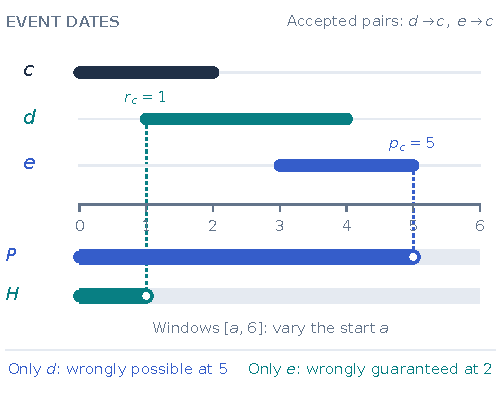
\includegraphics[width=\columnwidth]{figures/two_witnesses.pdf}
\caption{Two witnesses control different boundaries. Witness $d$ supplies $r_c=1$, while $e$ supplies $p_c=5$. The strips show support for windows $[a,6]$. Open endpoints exclude equality. Removing $e$ wrongly permits point 5; removing $d$ wrongly guarantees point 2.}
\label{fig:compiler}
\end{figure}

Let $n$ count modeled events, including explicit ends, and $m$ count accepted pairs.
Compilation takes $O(n+m)$ time and stores $O(n)$ certificate records.
Pair discovery remains the source adapter's responsibility.
The reference complete scan makes $n(n-1)$ gate calls.
An index can replace this scan when it preserves every accepted pair.

\subsection{An exact stability test}

Let $\pi_q$ be a complete relevance ranking for question $q$, including all tie breaks.
For a set $S$, write $\operatorname{Top}_k(S)$ for its first $k$ ranked claims.
Let $\mathcal W$ be any nonempty family of feasible timelines.
Define $P(Q)$ and $H(Q)$ by possible and guaranteed support over $\mathcal W$.
Only displayable claims enter these support sets.
The fast compiler uses $\mathcal W=\Omega$.
A realized timeline $x$ supplies a support set $S_x(Q)$.
The reader's selected claim context is
\begin{equation}
 R_x(q)=\operatorname{Top}_k(S_x(Q)).
\label{eq:context}
\end{equation}
Filtering preserves the ranking and occurs before the budget.

\begin{theorem}[Exact context stability]
\label{thm:context-stability}
For any nonempty family of feasible timelines, every timeline returns the same context exactly when
\begin{equation}
 \operatorname{Top}_k(P(Q))=\operatorname{Top}_k(H(Q)).
\label{eq:context-stability}
\end{equation}
Equivalently, every selected possible claim has guaranteed support.
\end{theorem}
\begin{proof}
Set $C=\operatorname{Top}_k(P(Q))$.
If $C\subseteq H(Q)$, every world retains $C$ and selects the same context.
Otherwise, choose $c\in C\setminus H(Q)$.
Some world supports $c$, while another does not.
At most $k-1$ possible claims outrank $c$.
Every world supporting $c$ therefore selects it.
The two worlds return different contexts.
For $k=0$, every context is empty.
\end{proof}

The theorem depends on fixed ranking and exact support masks.
It applies to dependent dates and other support predicates.
Only the support solver changes.
The test uses two filtered rankings without enumerating attainable contexts.
Let $F$ contain the fixed fallback excerpts.
Apply the test to $P(Q)\cup F$ and $H(Q)\cup F$.
Their inclusion remains constant while modeled dates vary.
Claim selection precedes source rendering and any word-budget truncation.
We report rendered-context agreement separately.

\paragraph{Choose a stable context budget.}
Let $r$ be the position of the first unresolved claim in the ranking of $P(Q)\cup F$.
Every budget $k<r$ returns a fixed context, while every $k\ge r$ permits a context change.
If no unresolved claim exists, every budget is stable.
The claim at position $r$ supplies a counterexample for every larger budget.
The system reports this stable prefix alongside the source dates requiring refinement.

\paragraph{Stop once the context is full.}
The implementation evaluates certificates lazily during selection.
It scans ranked candidates until $k$ possible excerpts fill the context.
It checks guaranteed support only for selected modeled claims.
Fixed fallback excerpts remain eligible without a temporal lookup.
If selection examines $j$ candidates, selection and certification take $O(j)$ time.
Other dates need no evaluation for this decision.

\subsection{Constructing and resolving an unstable context}
Let $U=\operatorname{Top}_k(P(Q)\cup F)\setminus(H(Q)\cup F)$.
These claims have unresolved support and enter the possible context.
Their status determines whether date uncertainty can change retrieval.

\begin{theorem}[Constructive instability and refinement]
\label{thm:refinement}
Under independent date bounds, if $U\ne\varnothing$, we construct two complete date assignments with different contexts in $O(n)$ time.
Here, $n$ counts the event dates.
Any stabilizing date refinement makes each claim in $U$ guaranteed or impossible.
\end{theorem}

Each $c\in U$ has fewer than $k$ possible claims above it.
Any timeline supporting $c$ therefore selects it.
We place each accepted replacement of $c$ no later than $c$ or after a supporting query time.
A second timeline places $c$ after the query, or a direct witness by the query start.
Date refinement can only remove possible claims.
Thus a remaining possible pivot cannot leave the possible context through rank changes.
It must become guaranteed.
The assignments use only event bounds and the compact certificate.
Let $N$ count ranked excerpts, including fallback text.
Full context replay takes $O(n+m+N)$ time with the accepted pair list.
Appendix~\ref{app:refinement} gives the construction and proof.

The witnesses locate the start or replacement date requiring refinement.
New unresolved claims can enter after current pivots disappear, so refinement recomputes the frontier.

\subsection{A tractability boundary}
Possible support concerns one claim at a time.
Possible context membership also depends on which higher-ranked claims coexist.
We ask whether a given claim enters the context under \emph{any} allowed timeline.
\begin{theorem}[Possible context membership]
\label{thm:hardness}
Possible context membership is NP-hard when $k$ is input; this result does not cover the fixed budget $k=5$.
\end{theorem}
The reduction uses a point query and a bipartite gate with one edge layer.
Appendix~\ref{app:hardness} gives the proof.

The appendix also gives a reduction with every start no later than the query.
Our stability test instead needs one unresolved claim inside the possible prefix.
Its rank guarantees selection whenever it has support.
The test needs only individual support, even when shared events couple claim eligibility.
Under independent bounds, this certifies stability without computing every attainable context member.


\subsection{Enforce known order only where it matters}
\label{sec:constrained}
A source can state that one appointment follows another without identifying either exact date.
We represent these dependencies as difference constraints, following temporal constraint networks~\citep{dechter1991temporal}.
This extension uses integer calendar days.
For example, $x_i-x_j\leq-1$ states that event $i$ precedes event $j$.
A departure date $z_c$ satisfies $x_c-z_c\leq-1$ and supplies a replacement pair targeting $c$.
This permits overlapping start and end bounds while retaining only valid lifetimes.
We check that the resulting feasible family $\Omega_D\subseteq\Omega$ is nonempty.

\paragraph{Select the query predicate.}
The interface distinguishes three temporal meanings.
Query meaning is an explicit input.
Overlap asks whether the claim applies somewhere in $[a,b]$.
Throughout asks whether it applies at every date in that window.
Appointment asks whether its start belongs to the window.
Let $D(c)=\{d:G(d,c)=1\}$.
The first two predicates have the common form
\begin{equation}
 x_c\leq s\ \land\!\bigwedge_{d\in D(c)}
 (x_d\leq x_c\ \lor\ x_d>t),
 \label{eq:constrained-support}
\end{equation}
where $(s,t)=(b,a)$ for overlap and $(a,b)$ for throughout.
Appointment instead requires $a\leq x_c\leq b$.

An exact oracle searches feasible branches of Equation~\ref{eq:constrained-support} and its negation.
It returns supporting and excluding timelines when they exist.
Possible support requires the former; guaranteed support excludes the latter.
Each branch uses standard difference-constraint feasibility.
Appendix~\ref{app:constrained-dates} proves completeness and gives the branching cost.
The context criterion in Theorem~\ref{thm:context-stability} then applies without changing the ranking.

\paragraph{Screen first, solve selectively.}
For overlap, let $P_0,H_0$ denote the independent compiler's support sets.
Let $P_D,H_D$ denote their exact constrained counterparts.
Restricting the timeline family gives
\begin{equation}
 H_0\subseteq H_D\subseteq P_D\subseteq P_0.
\end{equation}
Equal product contexts therefore certify the constrained context without any query-level oracle call.
Otherwise, scan the fixed ranking and skip claims outside $P_0$.
Accept claims in $H_0$ as guaranteed.
Query the exact oracle for remaining candidates until $k$ possible claims fill the context.
Fixed fallback excerpts extend this scan by entering every support set without an oracle call.
The resulting context is $\operatorname{Top}_k(P_D\cup F)$.
An unresolved selected claim supplies the two replayable timelines.

